\documentclass[12pt,a4paper]{article}
\usepackage[utf8]{inputenc}
\usepackage{amsmath}
\usepackage{amsfonts}
\usepackage{amssymb}
\usepackage[left=3cm,right=3cm,top=3cm,bottom=3cm]{geometry}
\usepackage{tikz}
\usetikzlibrary{arrows.meta}


\tikzset{
%->,  
%>=stealth, 
node distance=2.5cm, 
every state/.style={thick, fill=gray!10},  
auto,
}
\tikzstyle{every path}=[line width=0.8pt]

\title{Diagrams}




\begin{document}


\section{Model categories}


\begin{center}
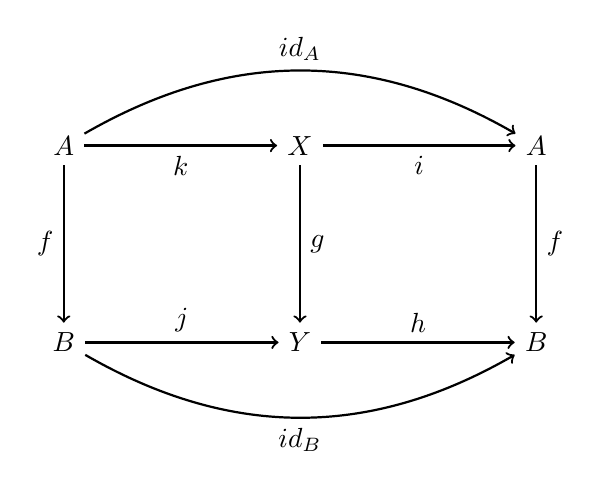
\begin{tikzpicture}
	\node (1) {$A$};
	\node (2) [below of=1] {$B$};
	\node (3) [node distance=3cm, right of=1] {$X$};
	\node (4) [below of=3] {$Y$};
	\node (5) [node distance=3cm, right of=3]{$A$};
	\node (6) [below of=5] {$B$};
	
	\draw [-to] (1) to node [swap]{$f$} (2);
	\draw [-to] (1) to node [swap]{$k$} (3);
	\draw [-to] (2) to node {$j$} (4);
	\draw [-to] (3) to node {$g$} (4);
	\draw [-to] (5) to node {$f$} (6);
	\draw [-to] (4) to node {$h$} (6);
	\draw [-to] (3) to node [swap]{$i$} (5);
	\draw [-to, bend left] (1) to node {$id_A$} (5);
	\draw [-to, bend right] (2) to node [swap] {$id_B$} (6);	
\end{tikzpicture}
\end{center}

\begin{center}
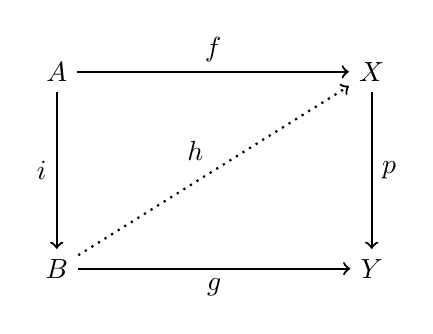
\begin{tikzpicture}
	\node (1) {$A$};
	\node (3) [below of=1] {$B$};
	\node (2) [node distance=4cm, right of=1] {$X$};
	\node (4) [below of=2] {$Y$};

	\draw [-to] (1) to node {$f$} (2);
	\draw [-to] (1) to node [swap]{$i$} (3);
	\draw [-to] (2) to node {$p$} (4);
	\draw [-to] (3) to node [swap]{$g$} (4);	
	\draw [-to, dotted] (3) to node {$h$} (2);
\end{tikzpicture}
\end{center}

\begin{center}
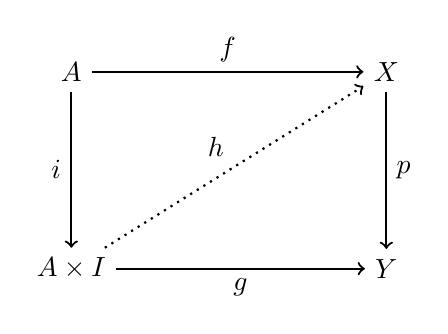
\begin{tikzpicture}
	\node (1) {$A$};
	\node (3) [below of=1] {$A\times I$};
	\node (2) [node distance=4cm, right of=1] {$X$};
	\node (4) [below of=2] {$Y$};

	\draw [-to] (1) to node {$f$} (2);
	\draw [-to] (1) to node [swap]{$i$} (3);
	\draw [-to] (2) to node {$p$} (4);
	\draw [-to] (3) to node [swap]{$g$} (4);	
	\draw [-to, dotted] (3) to node {$h$} (2);
\end{tikzpicture}
\end{center}

\begin{center}
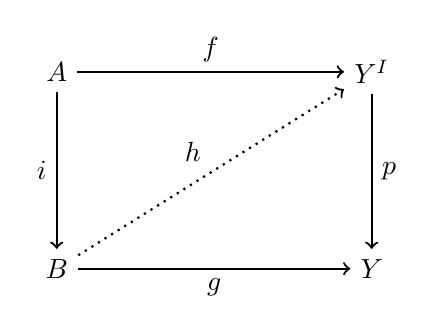
\begin{tikzpicture}
	\node (1) {$A$};
	\node (3) [below of=1] {$B$};
	\node (2) [node distance=4cm, right of=1] {$Y^I$};
	\node (4) [below of=2] {$Y$};

	\draw [-to] (1) to node {$f$} (2);
	\draw [-to] (1) to node [swap]{$i$} (3);
	\draw [-to] (2) to node {$p$} (4);
	\draw [-to] (3) to node [swap]{$g$} (4);	
	\draw [-to, dotted] (3) to node {$h$} (2);
\end{tikzpicture}
\end{center}

\begin{center}
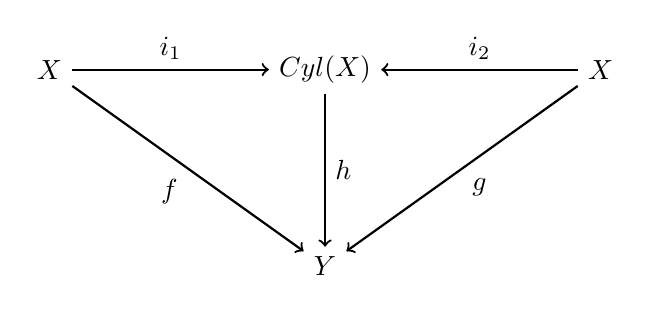
\begin{tikzpicture}
	\node (X) {$X$};
	\node (C) [node distance=3.5cm, right of=X] {$Cyl(X)$};
	\node (X') [node distance=3.5cm, right of=C] {$X$};
	\node (Y) [below of=C] {$Y$};

	\draw [-to] (X) to node {$i_1$} (C);
	\draw [-to] (X') to node [swap]{$i_2$} (C);
	\draw [-to] (X) to node [swap]{$f$} (Y);
	\draw [-to] (X') to node {$g$} (Y);
	\draw [-to] (C) to node {$h$} (Y);
\end{tikzpicture}
\end{center}

\begin{center}
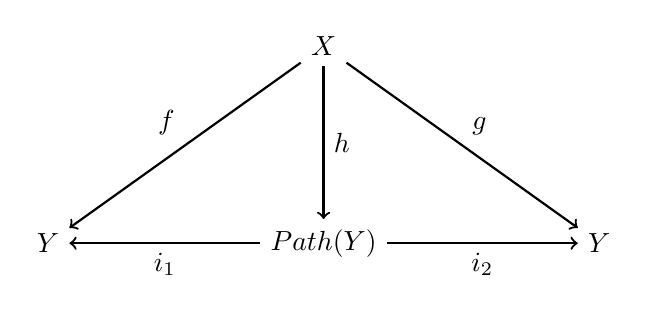
\begin{tikzpicture}
	\node (Y) {$Y$};
	\node (P) [node distance=3.5cm, right of=Y] {$Path(Y)$};
	\node (Y') [node distance=3.5cm, right of=P] {$Y$};
	\node (X) [above of=P] {$X$};

	\draw [-to] (X) to node [swap]{$f$} (Y);
	\draw [-to] (X) to node {$g$} (Y');
	\draw [-to] (X) to node {$h$} (P);
	\draw [-to] (P) to node {$i_1$} (Y);
	\draw [-to] (P) to node [swap]{$i_2$} (Y');
\end{tikzpicture}
\end{center}

\begin{center}
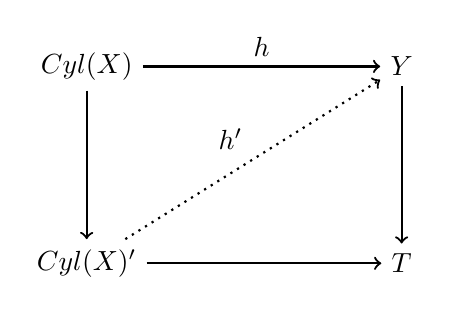
\begin{tikzpicture}
	\node (C) {$Cyl(X)$};
	\node (C') [below of=C] {$Cyl(X)'$};
	\node (Y) [node distance=4cm, right of=C] {$Y$};
	\node (T) [below of=Y] {$T$};

	\draw [-to] (C) to node {$h$} (Y);
	\draw [-to] (C) to node {} (C');
	\draw [-to] (C') to node {} (T);
	\draw [-to] (Y) to node {} (T);	
	\draw [-to, dotted] (C') to node {$h'$} (Y);
\end{tikzpicture}
\end{center}

\begin{center}
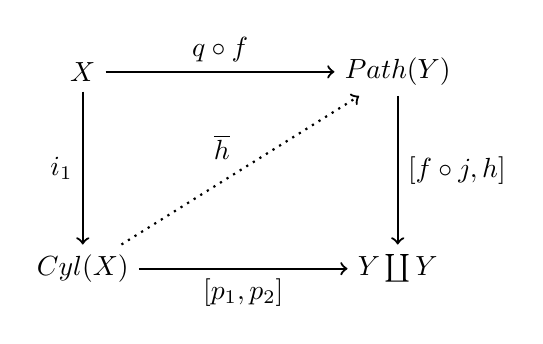
\begin{tikzpicture}
	\node (X) {$X$};
	\node (C) [below of=X] {$Cyl(X)$};
	\node (P) [node distance=4cm, right of=X] {$Path(Y)$};
	\node (Y) [below of=P] {$Y\coprod Y$};

	\draw [-to] (X) to node {$q\circ f$} (P);
	\draw [-to] (X) to node [swap]{$i_1$} (C);
	\draw [-to] (C) to node [swap]{$[p_1, p_2]$} (Y);
	\draw [-to] (P) to node {$[f\circ j, h]$} (Y);	
	\draw [-to, dotted] (C) to node {$\overline{h}$} (P);
\end{tikzpicture}
\end{center}

\begin{center}
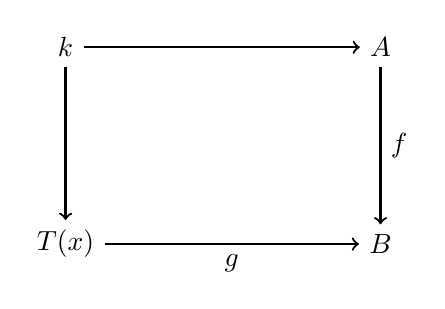
\begin{tikzpicture}
	\node (1) {$k$};
	\node (2) [below of=1] {$T(x)$};
	\node (3) [node distance=4cm, right of=1] {$A$};
	\node (4) [below of=3] {$B$};

	\draw [-to] (1) to node {} (2);
	\draw [-to] (1) to node {} (3);
	\draw [-to] (2) to node [swap]{$g$} (4);
	\draw [-to] (3) to node {$f$} (4);	
\end{tikzpicture}
\end{center}

\begin{center}
\begin{tikzpicture}
	\node (1) {$k$};
	\node (2) [below of=1] {$T(x)$};
	\node (3) [node distance=4cm, right of=1] {$A$};

	\draw [-to] (1) to node {} (2);
	\draw [-to] (1) to node {} (3);
\end{tikzpicture}
\end{center}

\begin{center}
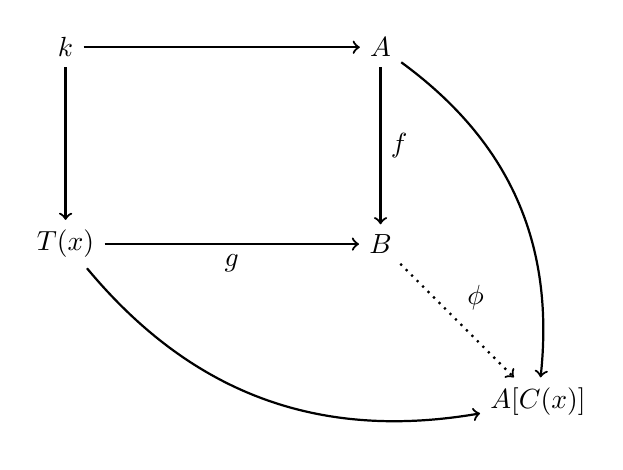
\begin{tikzpicture}
	\node (1) {$k$};
	\node (2) [below of=1] {$T(x)$};
	\node (3) [node distance=4cm, right of=1] {$A$};
	\node (4) [below of=3] {$B$};
	\node (5) [node distance=2cm, right of=4, below of=4] {$A[C(x)]$};

	\draw [-to] (1) to node {} (2);
	\draw [-to] (1) to node {} (3);
	\draw [-to] (2) to node [swap]{$g$} (4);
	\draw [-to] (3) to node {$f$} (4);	
	\draw [-to, dotted] (4) to node {$\phi$} (5);
	\draw [-to, bend left] (3) to node {} (5);
	\draw [-to, bend right] (2) to node {} (5);
\end{tikzpicture}
\end{center}

\begin{center}
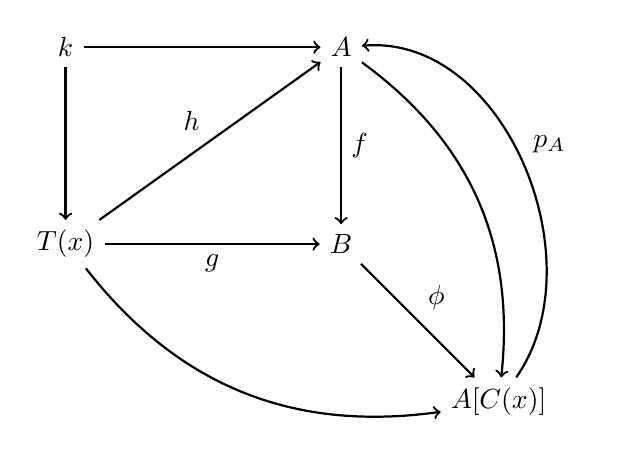
\begin{tikzpicture}
	\node (1) {$k$};
	\node (2) [below of=1] {$T(x)$};
	\node (3) [node distance=3.5cm, right of=1] {$A$};
	\node (4) [below of=3] {$B$};
	\node (5) [node distance=2cm, right of=4, below of=4] {$A[C(x)]$};

	\draw [-to] (1) to node {} (2);
	\draw [-to] (1) to node {} (3);
	\draw [-to] (2) to node [swap]{$g$} (4);
	\draw [-to] (3) to node {$f$} (4);	
	\draw [-to] (2) to node {$h$} (3);
	\draw [-to] (4) to node {$\phi$} (5);
	\draw [-to, bend left] (3) to node {} (5);
	\draw [-to, bend right] (2) to node {} (5);
	\draw [-to, bend right, in=250, out=300] (5) to node [swap]{$p_A$} (3);
\end{tikzpicture}
\end{center}

\begin{center}
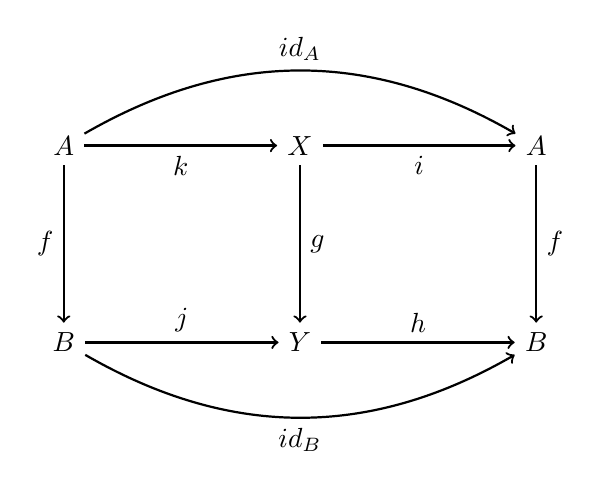
\begin{tikzpicture}
	\node (1) {$A$};
	\node (2) [below of=1] {$B$};
	\node (3) [node distance=3cm, right of=1] {$X$};
	\node (4) [below of=3] {$Y$};
	\node (5) [node distance=3cm, right of=3]{$A$};
	\node (6) [below of=5] {$B$};
	
	\draw [-to] (1) to node [swap]{$f$} (2);
	\draw [-to] (1) to node [swap]{$k$} (3);
	\draw [-to] (2) to node {$j$} (4);
	\draw [-to] (3) to node {$g$} (4);
	\draw [-to] (5) to node {$f$} (6);
	\draw [-to] (4) to node {$h$} (6);
	\draw [-to] (3) to node [swap]{$i$} (5);
	\draw [-to, bend left] (1) to node {$id_A$} (5);
	\draw [-to, bend right] (2) to node [swap] {$id_B$} (6);	
\end{tikzpicture}
\end{center}

\begin{center}
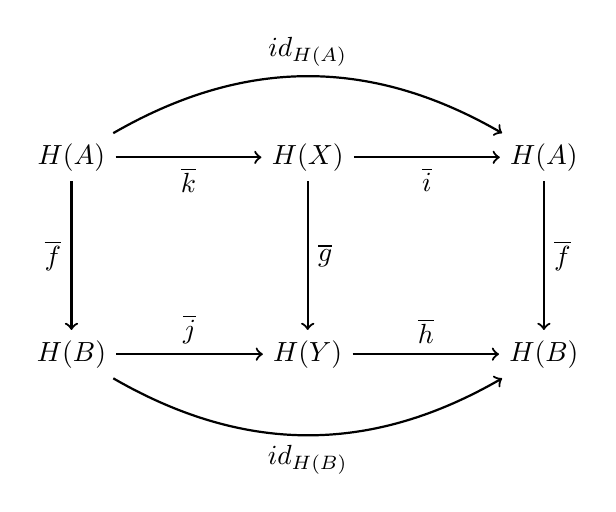
\begin{tikzpicture}
	\node (1) {$H(A)$};
	\node (2) [below of=1] {$H(B)$};
	\node (3) [node distance=3cm, right of=1] {$H(X)$};
	\node (4) [below of=3] {$H(Y)$};
	\node (5) [node distance=3cm, right of=3]{$H(A)$};
	\node (6) [below of=5] {$H(B)$};
	
	\draw [-to] (1) to node [swap]{$\overline{f}$} (2);
	\draw [-to] (1) to node [swap]{$\overline{k}$} (3);
	\draw [-to] (2) to node {$\overline{j}$} (4);
	\draw [-to] (3) to node {$\overline{g}$} (4);
	\draw [-to] (5) to node {$\overline{f}$} (6);
	\draw [-to] (4) to node {$\overline{h}$} (6);
	\draw [-to] (3) to node [swap]{$\overline{i}$} (5);
	\draw [-to, bend left] (1) to node {$id_{H(A)}$} (5);
	\draw [-to, bend right] (2) to node [swap] {$id_{H(B)}$} (6);	
\end{tikzpicture}
\end{center}

\begin{center}
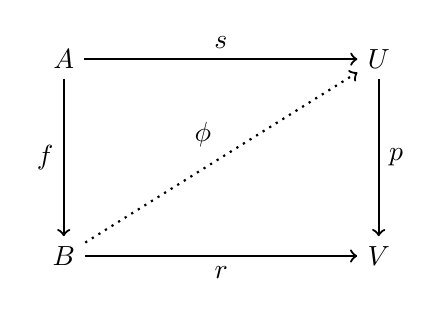
\begin{tikzpicture}
	\node (1) {$A$};
	\node (2) [node distance=4cm, right of=1] {$U$};
	\node (3) [below of=1] {$B$};
	\node (4) [below of=2] {$V$};

	\draw [-to] (1) to node {$s$} (2);
	\draw [-to] (1) to node [swap]{$f$} (3);
	\draw [-to] (2) to node {$p$} (4);
	\draw [-to] (3) to node [swap]{$r$} (4);	
	\draw [-to, dotted] (3) to node {$\phi$} (2);
\end{tikzpicture}
\end{center}

\begin{center}
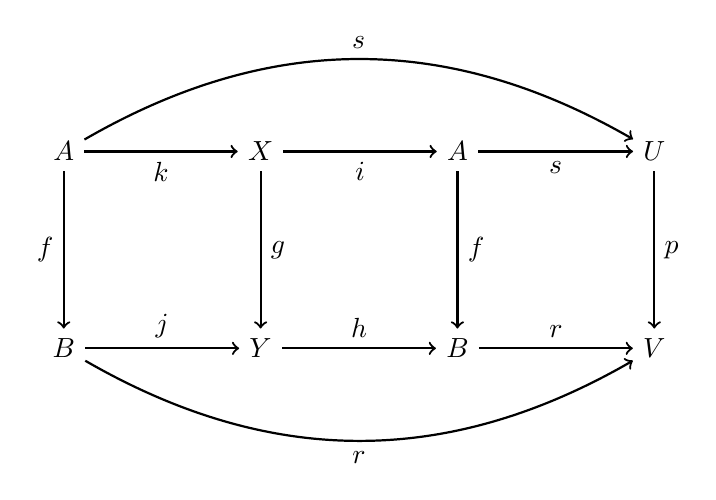
\begin{tikzpicture}
	\node (1) {$A$};
	\node (2) [right of=1] {$X$};	
	\node (3) [right of=2]{$A$};	
	\node (4) [right of=3] {$U$};	
	
	\node (5) [below of=1] {$B$};
	\node (6) [below of=2] {$Y$};
	\node (7) [below of=3] {$B$};
	\node (8) [below of=4] {$V$};
	
	\draw [-to] (1) to node [swap]{$f$} (5);
	\draw [-to] (1) to node [swap]{$k$} (2);
	\draw [-to] (5) to node {$j$} (6);
	\draw [-to] (2) to node {$g$} (6);
	\draw [-to] (3) to node {$f$} (7);
	\draw [-to] (6) to node {$h$} (7);
	\draw [-to] (2) to node [swap]{$i$} (3);
	\draw [-to] (3) to node [swap]{$s$} (4);
	\draw [-to] (7) to node {$r$} (8);	
	\draw [-to] (4) to node {$p$} (8);	
	\draw [-to, bend left] (1) to node {$s$} (4);
	\draw [-to, bend right] (5) to node [swap]{$r$} (8);	
\end{tikzpicture}
\end{center}

\begin{center}
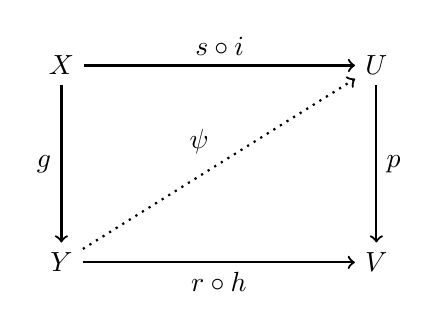
\begin{tikzpicture}
	\node (1) {$X$};
	\node (2) [node distance=4cm, right of=1] {$U$};
	\node (3) [below of=1] {$Y$};
	\node (4) [below of=2] {$V$};

	\draw [-to] (1) to node {$s\circ i$} (2);
	\draw [-to] (1) to node [swap]{$g$} (3);
	\draw [-to] (2) to node {$p$} (4);
	\draw [-to] (3) to node [swap]{$r\circ h$} (4);	
	\draw [-to, dotted] (3) to node {$\psi$} (2);
\end{tikzpicture}
\end{center}

\begin{center}
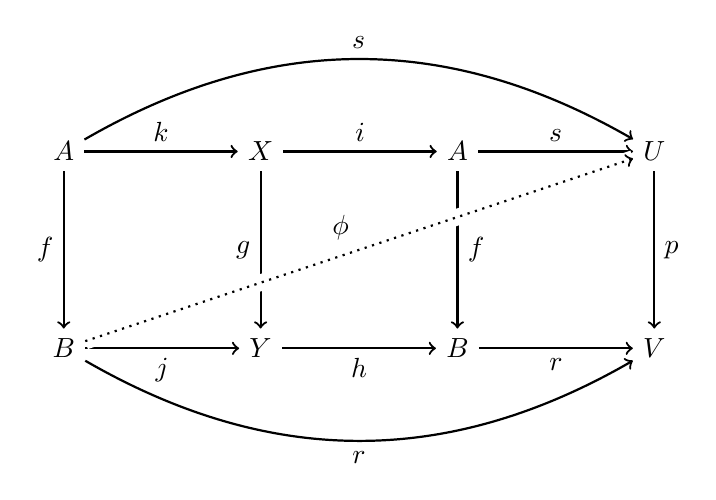
\begin{tikzpicture}[%
	cross line/.style={preaction={draw=white, -,line width=6pt}}]
	\node (1) {$A$};
	\node (2) [right of=1] {$X$};	
	\node (3) [right of=2]{$A$};	
	\node (4) [right of=3] {$U$};	
	
	\node (5) [below of=1] {$B$};
	\node (6) [below of=2] {$Y$};
	\node (7) [below of=3] {$B$};
	\node (8) [below of=4] {$V$};
	
	\draw [-to] (1) to node [swap]{$f$} (5);
	\draw [-to] (1) to node {$k$} (2);
	\draw [-to] (5) to node [swap]{$j$} (6);
	\draw [-to] (2) to node [swap]{$g$} (6);
	\draw [-to] (3) to node {$f$} (7);
	\draw [-to] (6) to node [swap]{$h$} (7);
	\draw [-to] (2) to node {$i$} (3);
	\draw [-to] (3) to node {$s$} (4);
	\draw [-to] (7) to node [swap]{$r$} (8);	
	\draw [-to] (4) to node {$p$} (8);	
	\draw [-to, bend left] (1) to node {$s$} (4);
	\draw [-to, bend right] (5) to node [swap]{$r$} (8);	
	\draw [-to, cross line, dotted] (5) to node {$\phi$} (4);
	
\end{tikzpicture}
\end{center}

\begin{center}
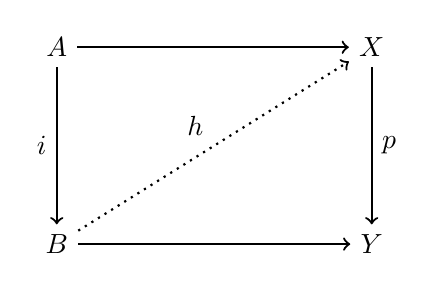
\begin{tikzpicture}
	\node (1) {$A$};
	\node (3) [below of=1] {$B$};
	\node (2) [node distance=4cm, right of=1] {$X$};
	\node (4) [below of=2] {$Y$};

	\draw [-to] (1) to node {} (2);
	\draw [-to] (1) to node [swap]{$i$} (3);
	\draw [-to] (2) to node {$p$} (4);
	\draw [-to] (3) to node [swap]{} (4);	
	\draw [-to, dotted] (3) to node {$h$} (2);
\end{tikzpicture}
\end{center}

\begin{center}
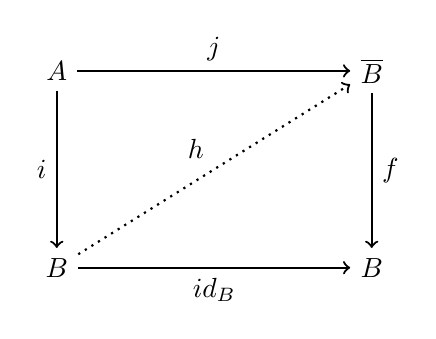
\begin{tikzpicture}
	\node (1) {$A$};
	\node (3) [below of=1] {$B$};
	\node (2) [node distance=4cm, right of=1] {$\overline{B}$};
	\node (4) [below of=2] {$B$};

	\draw [-to] (1) to node {$j$} (2);
	\draw [-to] (1) to node [swap]{$i$} (3);
	\draw [-to] (2) to node {$f$} (4);
	\draw [-to] (3) to node [swap]{$id_B$} (4);	
	\draw [-to, dotted] (3) to node {$h$} (2);
\end{tikzpicture}
\end{center}

\begin{center}
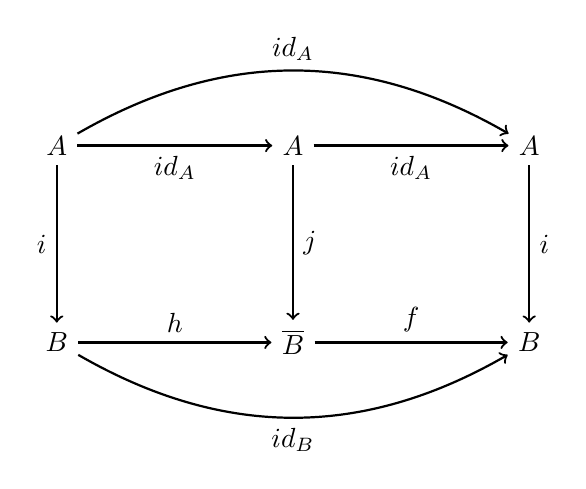
\begin{tikzpicture}
	\node (1) {$A$};
	\node (2) [below of=1] {$B$};
	\node (3) [node distance=3cm, right of=1] {$A$};
	\node (4) [below of=3] {$\overline{B}$};
	\node (5) [node distance=3cm, right of=3]{$A$};
	\node (6) [below of=5] {$B$};
	
	\draw [-to] (1) to node [swap]{$i$} (2);
	\draw [-to] (1) to node [swap]{$id_A$} (3);
	\draw [-to] (2) to node {$h$} (4);
	\draw [-to] (3) to node {$j$} (4);
	\draw [-to] (5) to node {$i$} (6);
	\draw [-to] (4) to node {$f$} (6);
	\draw [-to] (3) to node [swap]{$id_A$} (5);
	\draw [-to, bend left] (1) to node {$id_A$} (5);
	\draw [-to, bend right] (2) to node [swap] {$id_B$} (6);	
\end{tikzpicture}
\end{center}

\section{More formality}

\begin{center}
\begin{tikzpicture}
	\node (1) {$A$};
	\node (2) [right of=1] {$A_1$};
	\node (3) [right of=2] {$A_2$};
	\node (4) [right of=3] {$A_3$};
	\node (5) [right of=4] {$\cdots$};
	\node (6) [below of=2] {$C_1$};
	
	\draw [-to] (1) to node {$q_0$} (2);
	\draw [to-] (2) to node {$q_1$} (3);
	\draw [-to] (3) to node {$q_2$} (4);
	\draw [to-] (4) to node {} (5);
	\draw [-to] (6) to node {$p_0$} (1);
	\draw [-to] (6) to node [swap]{$p_1$} (3);	
\end{tikzpicture}
\end{center}

\begin{center}
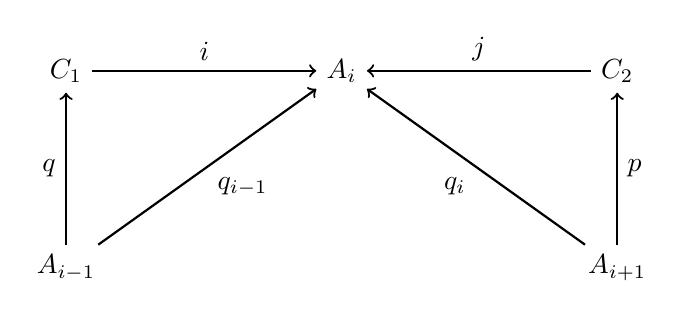
\begin{tikzpicture}
	\node (1) {$C_1$};
	\node (2) [node distance=3.5cm, right of=1] {$A_i$};
	\node (3) [node distance=3.5cm, right of=2] {$C_2$};
	\node (4) [below of=1] {$A_{i-1}$};
	\node (5) [below of=3] {$A_{i+1}$};
	
	\draw [-to] (1) to node {$i$} (2);
	\draw [to-] (2) to node {$j$} (3);
	\draw [-to] (4) to node [swap]{$q_{i-1}$} (2);
	\draw [-to] (5) to node {$q_i$} (2);
	\draw [-to] (4) to node {$q$} (1);
	\draw [-to] (5) to node [swap]{$p$} (3);		
\end{tikzpicture}
\end{center}

\begin{center}
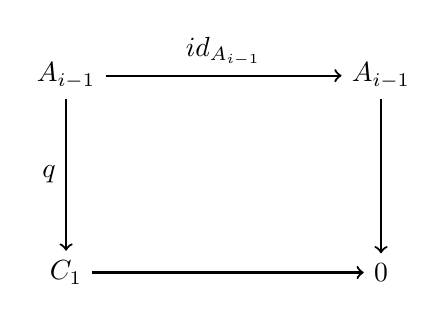
\begin{tikzpicture}
	\node (1) {$A_{i-1}$};
	\node (2) [node distance=4cm, right of=1] {$A_{i-1}$};	
	\node (3) [below of=1] {$C_1$};
	\node (4) [below of=2] {$0$};

	\draw [-to] (1) to node {$id_{A_{i-1}}$} (2);
	\draw [-to] (1) to node [swap]{$q$} (3);
	\draw [-to] (2) to node {} (4);
	\draw [-to] (3) to node {} (4);	
\end{tikzpicture}
\end{center}

\begin{center}
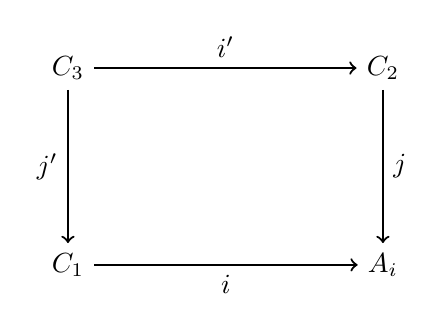
\begin{tikzpicture}
	\node (1) {$C_3$};
	\node (2) [node distance=4cm, right of=1] {$C_2$};	
	\node (3) [below of=1] {$C_1$};
	\node (4) [below of=2] {$A_i$};

	\draw [-to] (1) to node {$i'$} (2);
	\draw [-to] (1) to node [swap]{$j'$} (3);
	\draw [-to] (2) to node {$j$} (4);
	\draw [-to] (3) to node [swap]{$i$} (4);	
\end{tikzpicture}
\end{center}

\begin{center}
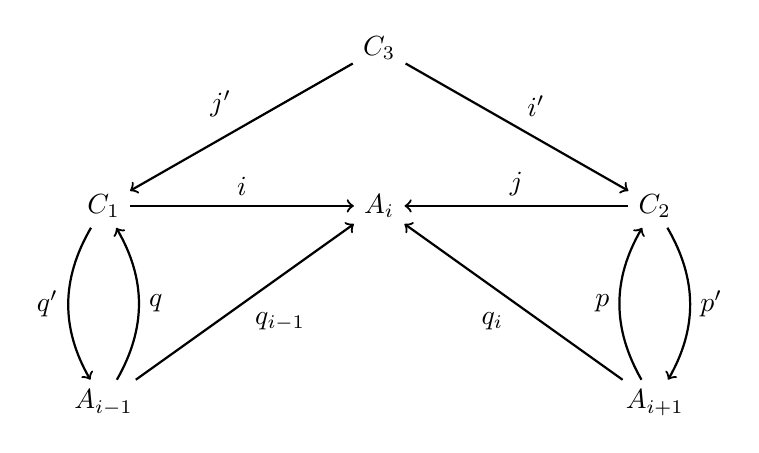
\begin{tikzpicture}
	\node (1) {$C_1$};
	\node (2) [node distance=3.5cm, right of=1] {$A_i$};
	\node (3) [node distance=3.5cm, right of=2] {$C_2$};
	\node (4) [below of=1] {$A_{i-1}$};
	\node (5) [below of=3] {$A_{i+1}$};
	\node (6) [node distance=2cm, above of=2] {$C_3$};
	
	\draw [-to] (6) to node [swap]{$j'$} (1);
	\draw [-to] (6) to node {$i'$} (3);
	\draw [-to] (1) to node {$i$} (2);
	\draw [to-] (2) to node {$j$} (3);
	\draw [-to] (4) to node [swap]{$q_{i-1}$} (2);
	\draw [-to] (5) to node {$q_i$} (2);
	\draw [-to, bend right] (4) to node [swap]{$q$} (1);
	\draw [-to, bend left] (5) to node {$p$} (3);	
	\draw [to-, bend left] (4) to node {$q'$} (1);
	\draw [to-, bend right] (5) to node [swap]{$p'$} (3);				
\end{tikzpicture}
\end{center}

\begin{center}
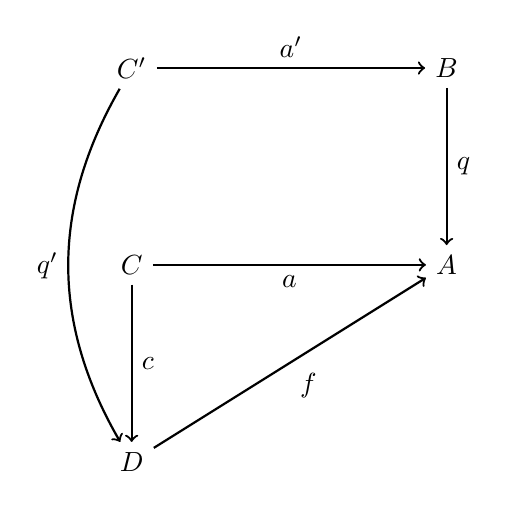
\begin{tikzpicture}
	\node (1) {$C'$};
	\node (2) [node distance=4cm, right of=1] {$B$};	
	\node (3) [below of=1] {$C$};
	\node (4) [below of=2] {$A$};
	\node (5) [below of=3] {$D$};

	\draw [-to] (1) to node {$a'$} (2);
	\draw [-to, bend right] (1) to node [swap]{$q'$} (5);
	\draw [-to] (2) to node {$q$} (4);
	\draw [-to] (3) to node [swap]{$a$} (4);
	\draw [-to] (3) to node {$c$} (5);
	\draw [-to] (5) to node [swap]{$f$} (4);
\end{tikzpicture}
\end{center}

\begin{center}
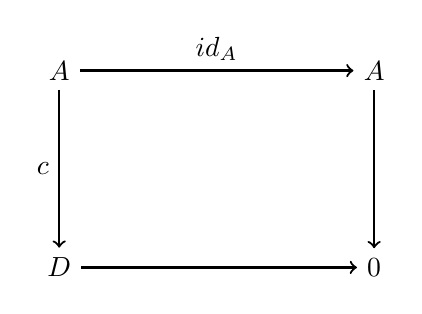
\begin{tikzpicture}
	\node (1) {$A$};
	\node (2) [node distance=4cm, right of=1] {$A$};	
	\node (3) [below of=1] {$D$};
	\node (4) [below of=2] {$0$};

	\draw [-to] (1) to node {$id_A$} (2);
	\draw [-to] (1) to node [swap]{$c$} (3);
	\draw [-to] (2) to node {} (4);
	\draw [-to] (3) to node {} (4);	
\end{tikzpicture}
\end{center}

\begin{center}
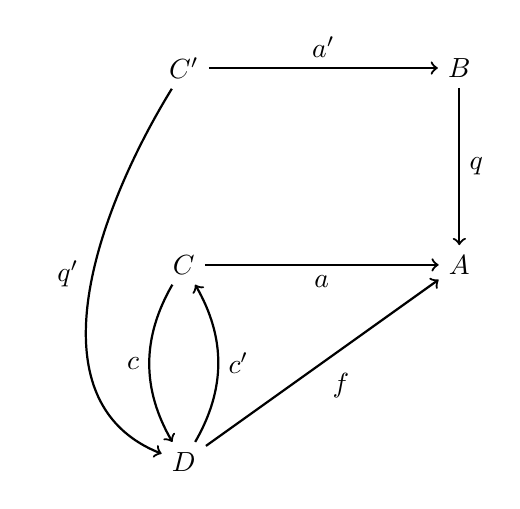
\begin{tikzpicture}
	\node (1) {$C'$};
	\node (2) [node distance=3.5cm, right of=1] {$B$};	
	\node (3) [below of=1] {$C$};
	\node (4) [below of=2] {$A$};
	\node (5) [below of=3] {$D$};

	\draw [-to] (1) to node {$a'$} (2);
	\draw [-to, bend right, in=250] (1) to node [swap]{$q'$} (5);
	\draw [-to] (2) to node {$q$} (4);
	\draw [-to] (3) to node [swap]{$a$} (4);
	\draw [-to, bend right] (3) to node [swap]{$c$} (5);
	\draw [to-, bend left] (3) to node {$c'$} (5);	
	\draw [-to] (5) to node [swap]{$f$} (4);
\end{tikzpicture}
\end{center}

\begin{center}
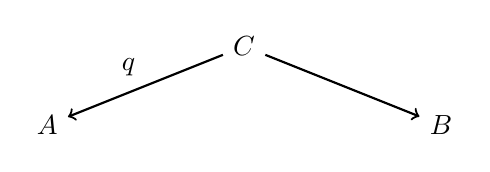
\begin{tikzpicture}
	\node (1) {$A$};
	\node (2) [right of=1] { };	
	\node (3) [right of=2] {$B$};	
	\node (4) [node distance=1cm, above of=2] {$C$};

	\draw [-to] (4) to node [swap]{$q$} (1);
	\draw [-to] (4) to node {} (3);
\end{tikzpicture}
\end{center}

\begin{center}
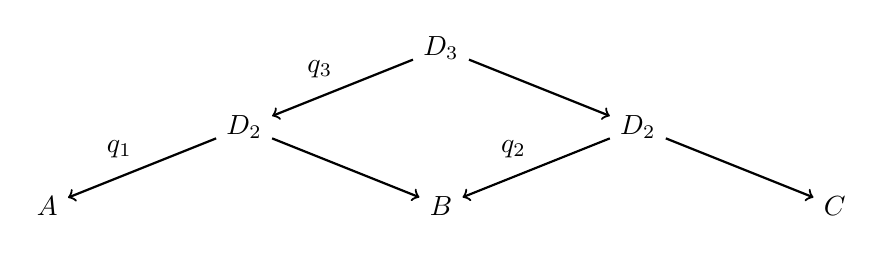
\begin{tikzpicture}
	\node (1) {$A$};
	\node (2) [right of=1] {};	
	\node (3) [right of=2] {$B$};	
	\node (4) [node distance=1cm, above of=2] {$D_2$};
	\node (5) [right of=3] {};
	\node (6) [right of=5] {$C$};
	\node (7) [node distance=1cm, above of=5] {$D_2$};
	\node (8) [right of=4] {};
	\node (9) [node distance=1cm, above of=8] {$D_3$};

	\draw [-to] (4) to node [swap]{$q_1$} (1);
	\draw [-to] (4) to node {} (3);
	\draw [-to] (7) to node [swap]{$q_2$} (3);
	\draw [-to] (7) to node {} (6);	
	\draw [-to] (9) to node [swap]{$q_3$} (4);
	\draw [-to] (9) to node {} (7);		
\end{tikzpicture}
\end{center}

\begin{center}
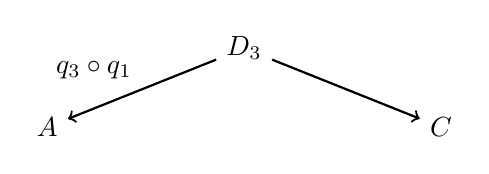
\begin{tikzpicture}
	\node (1) {$A$};
	\node (2) [right of=1] { };	
	\node (3) [right of=2] {$C$};	
	\node (4) [node distance=1cm, above of=2] {$D_3$};

	\draw [-to] (4) to node [swap]{$q_3\circ q_1$} (1);
	\draw [-to] (4) to node {} (3);
\end{tikzpicture}
\end{center}

\section{Deformation retraction}

\begin{center}
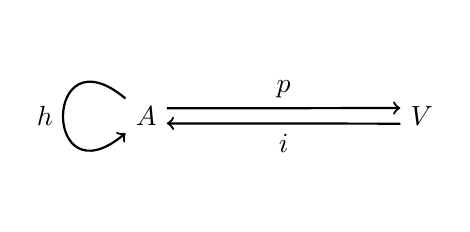
\begin{tikzpicture}
	\node (1) {$A$};
	\node (2) [node distance=3.5cm, right of=1] {$V$};
	
	\draw [to-, out=220, in=140, loop] (1) to node {$h$} (1);
	\draw [-to] (1.20) to node {$p$} (2.160);
	\draw [-to] (2.200) to node {$i$} (1.340);
\end{tikzpicture}
\end{center}

\begin{center}
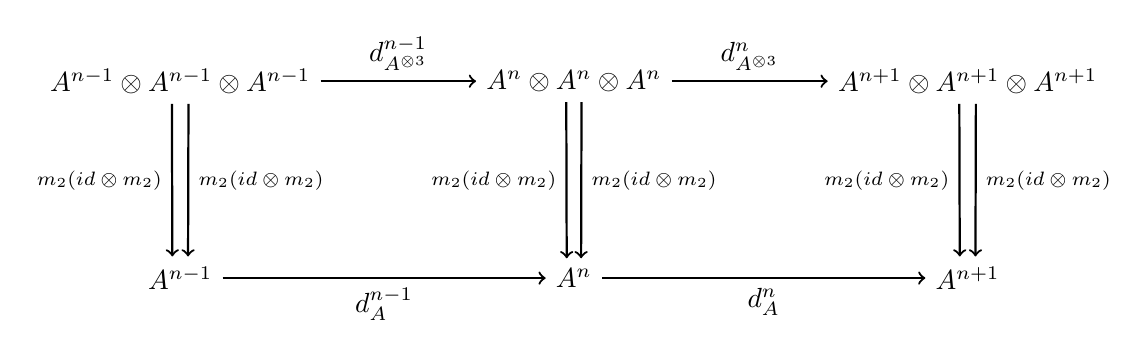
\begin{tikzpicture}
	\node (1) {$A^{n-1}\otimes A^{n-1}\otimes A^{n-1}$};
	\node (2) [node distance=5cm, right of=1] {$A^n\otimes A^n\otimes A^n$};
	\node (3) [node distance=5cm, right of=2] {$A^{n+1}\otimes A^{n+1}\otimes A^{n+1}$};
	
	\node (4) [below of=1] {$A^{n-1}$};
	\node (5) [node distance=5cm, right of=4] {$A^n$};
	\node (6) [node distance=5cm, right of=5] {$A^{n+1}$};

	\draw [-to] (1.250) to node [swap]{{\scriptsize $m_2(id\otimes m_2)$}} (4.110);
	\draw [-to] (1.290) to node {{\scriptsize $m_2(id\otimes m_2)$}} (4.70);
	\draw [-to] (2.250) to node [swap]{{\scriptsize $m_2(id\otimes m_2)$}} (5.110);
	\draw [-to] (2.290) to node {{\scriptsize $m_2(id\otimes m_2)$}} (5.70);
	\draw [-to] (3.250) to node [swap]{{\scriptsize $m_2(id\otimes m_2)$}} (6.110);
	\draw [-to] (3.290) to node {{\scriptsize $m_2(id\otimes m_2)$}} (6.70);
	\draw [-to] (1) to node {$d^{n-1}_{A^{\otimes 3}}$} (2);
	\draw [-to] (2) to node {$d^{n}_{A^{\otimes 3}}$} (3);
	\draw [-to] (4) to node [swap]{$d^{n-1}_{A}$} (5);
	\draw [-to] (5) to node [swap]{$d^{n}_{A}$} (6);
\end{tikzpicture}
\end{center}

\begin{center}
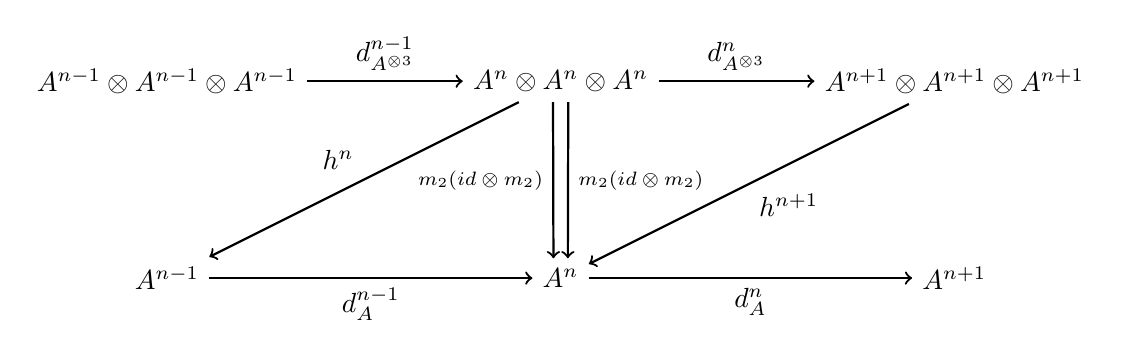
\begin{tikzpicture}
	\node (1) {$A^{n-1}\otimes A^{n-1}\otimes A^{n-1}$};
	\node (2) [node distance=5cm, right of=1] {$A^n\otimes A^n\otimes A^n$};
	\node (3) [node distance=5cm, right of=2] {$A^{n+1}\otimes A^{n+1}\otimes A^{n+1}$};
	
	\node (4) [below of=1] {$A^{n-1}$};
	\node (5) [node distance=5cm, right of=4] {$A^n$};
	\node (6) [node distance=5cm, right of=5] {$A^{n+1}$};

	\draw [-to] (2) to node [swap]{$h^n$} (4);
	\draw [-to] (3) to node {$h^{n+1}$} (5);
	\draw [-to] (2.250) to node [swap]{{\scriptsize $m_2(id\otimes m_2)$}} (5.110);
	\draw [-to] (2.290) to node {{\scriptsize $m_2(id\otimes m_2)$}} (5.70);
	\draw [-to] (1) to node {$d^{n-1}_{A^{\otimes 3}}$} (2);
	\draw [-to] (2) to node {$d^{n}_{A^{\otimes 3}}$} (3);
	\draw [-to] (4) to node [swap]{$d^{n-1}_{A}$} (5);
	\draw [-to] (5) to node [swap]{$d^{n}_{A}$} (6);
\end{tikzpicture}
\end{center}

\section{Kadeishvili's theorem}

\begin{center}
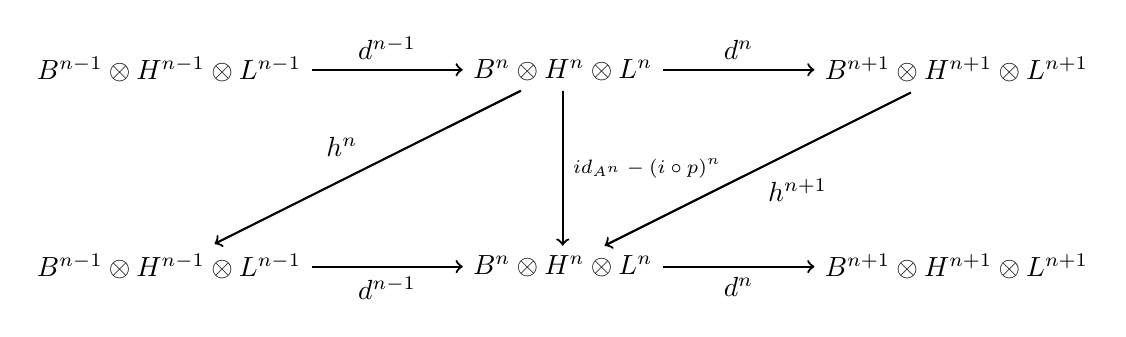
\begin{tikzpicture}
	\node (1) {$B^{n-1}\otimes H^{n-1}\otimes L^{n-1}$};
	\node (2) [node distance=5cm, right of=1] {$B^n\otimes H^n\otimes L^n$};
	\node (3) [node distance=5cm, right of=2] {$B^{n+1}\otimes H^{n+1}\otimes L^{n+1}$};
	
	\node (4) [below of=1]{$B^{n-1}\otimes H^{n-1}\otimes L^{n-1}$};
	\node (5) [node distance=5cm, right of=4] {$B^n\otimes H^n\otimes L^n$};
	\node (6) [node distance=5cm, right of=5] {$B^{n+1}\otimes H^{n+1}\otimes L^{n+1}$};

	\draw [-to] (2) to node [swap]{$h^n$} (4);
	\draw [-to] (3) to node {$h^{n+1}$} (5);
	\draw [-to] (2) to node {{\scriptsize $id_{A^n}-(i\circ p)^n$}} (5);
	
	\draw [-to] (1) to node {$d^{n-1}$} (2);
	\draw [-to] (2) to node {$d^{n}$} (3);
	\draw [-to] (4) to node [swap]{$d^{n-1}$} (5);
	\draw [-to] (5) to node [swap]{$d^{n}$} (6);
\end{tikzpicture}
\end{center}

\begin{center}
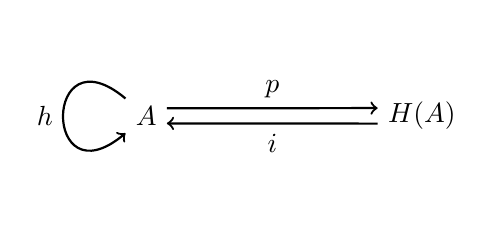
\begin{tikzpicture}
	\node (1) {$A$};
	\node (2) [node distance=3.5cm, right of=1] {$H(A)$};
	
	\draw [to-, out=220, in=140, loop] (1) to node {$h$} (1);
	\draw [-to] (1.20) to node {$p$} (2.170);
	\draw [-to] (2.190) to node {$i$} (1.340);
\end{tikzpicture}
\end{center}



\section{Lusternik-Schirelmann category 1 spaces}

\begin{center}
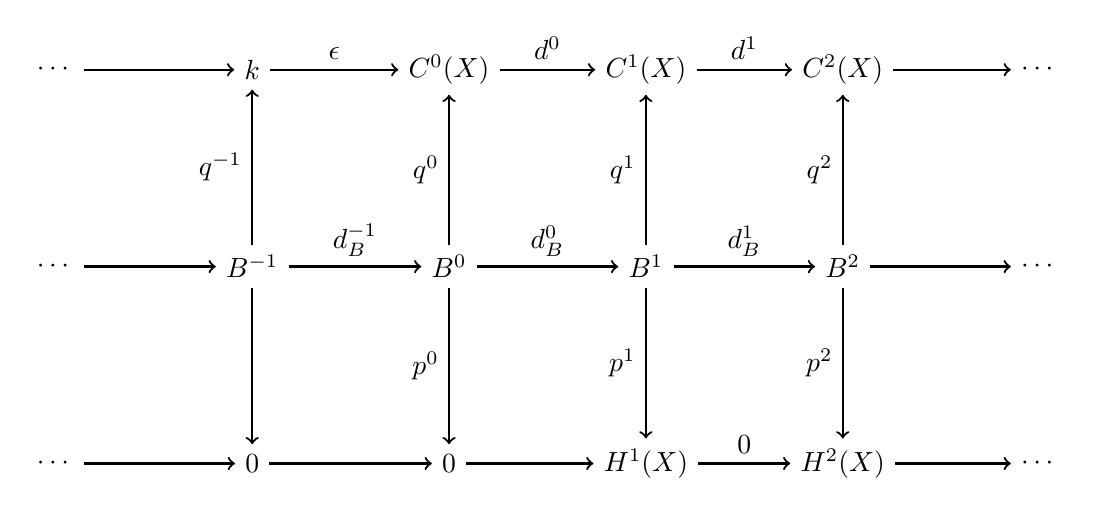
\begin{tikzpicture}
	\node (1) {$k$};
	\node (2) [right of=1] {$C^0(X)$};
	\node (3) [right of=2] {$C^1(X)$};
	\node (4) [right of=3] {$C^2(X)$};
	
	\node (5) [below of=1] {$B^{-1}$};
	\node (6) [right of=5] {$B^0$};
	\node (7) [right of=6] {$B^1$};
	\node (8) [right of=7] {$B^2$};
	
	\node (9) [below of=5] {$0$};
	\node (10) [right of=9] {$0$};
	\node (11) [right of=10] {$H^1(X)$};
	\node (12) [right of=11] {$H^2(X)$};
	
	\node (13) [left of=1] {$\cdots$};
	\node (14) [left of=5] {$\cdots$};
	\node (15) [left of=9] {$\cdots$};
	\node (16) [right of=4] {$\cdots$};
	\node (17) [right of=8] {$\cdots$};
	\node (18) [right of=12] {$\cdots$};
	
	\draw [-to] (13) to node {} (1);
	\draw [-to] (14) to node {} (5);
	\draw [-to] (15) to node {} (9);
	\draw [-to] (4) to node {} (16);
	\draw [-to] (8) to node {} (17);
	\draw [-to] (12) to node {} (18);
	
	\draw [-to] (1) to node {$\epsilon$} (2);
	\draw [-to] (2) to node {$d^0$} (3);
	\draw [-to] (3) to node {$d^1$} (4);
	
	\draw [-to] (5) to node {$d^{-1}_B$} (6);
	\draw [-to] (6) to node {$d^0_B$} (7);
	\draw [-to] (7) to node {$d^1_B$} (8);
	
	\draw [-to] (9) to node {} (10);
	\draw [-to] (10) to node {} (11);
	\draw [-to] (11) to node {$0$} (12);
	
	\draw [-to] (5) to node {$q^{-1}$} (1);
	\draw [-to] (5) to node {} (9);
	
	\draw [-to] (6) to node {$q^0$} (2);
	\draw [-to] (6) to node [swap]{$p^0$} (10);
	
	\draw [-to] (7) to node {$q^1$} (3);
	\draw [-to] (7) to node [swap]{$p^1$} (11);
	
	\draw [-to] (8) to node {$q^2$} (4);
	\draw [-to] (8) to node [swap]{$p^2$} (12);
\end{tikzpicture}
\end{center}

\begin{center}
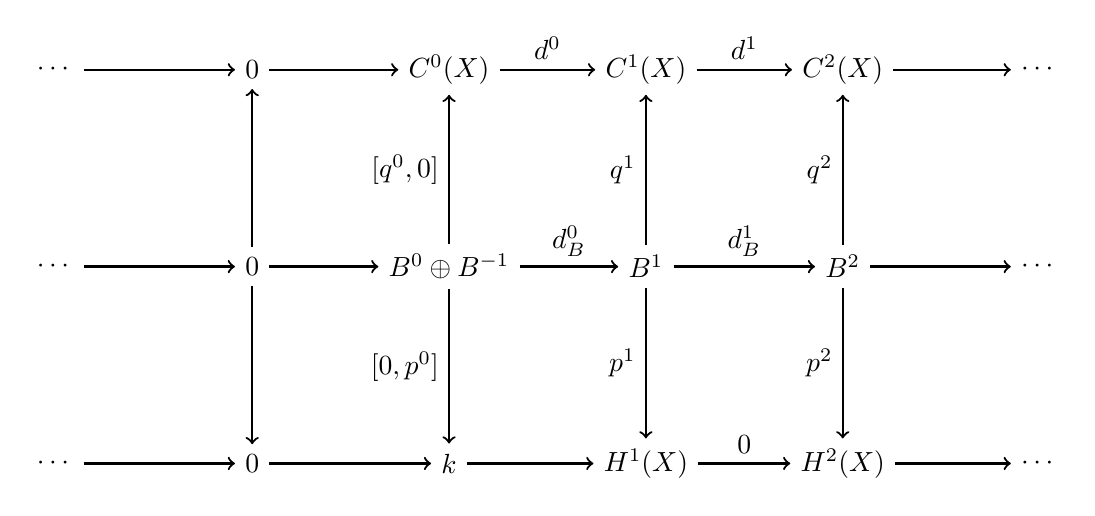
\begin{tikzpicture}
	\node (1) {$0$};
	\node (2) [right of=1] {$C^0(X)$};
	\node (3) [right of=2] {$C^1(X)$};
	\node (4) [right of=3] {$C^2(X)$};
	
	\node (5) [below of=1] {$0$};
	\node (6) [right of=5] {$B^0\oplus B^{-1}$};
	\node (7) [right of=6] {$B^1$};
	\node (8) [right of=7] {$B^2$};
	
	\node (9) [below of=5] {$0$};
	\node (10) [right of=9] {$k$};
	\node (11) [right of=10] {$H^1(X)$};
	\node (12) [right of=11] {$H^2(X)$};
	
	\node (13) [left of=1] {$\cdots$};
	\node (14) [left of=5] {$\cdots$};
	\node (15) [left of=9] {$\cdots$};
	\node (16) [right of=4] {$\cdots$};
	\node (17) [right of=8] {$\cdots$};
	\node (18) [right of=12] {$\cdots$};
	
	\draw [-to] (13) to node {} (1);
	\draw [-to] (14) to node {} (5);
	\draw [-to] (15) to node {} (9);
	\draw [-to] (4) to node {} (16);
	\draw [-to] (8) to node {} (17);
	\draw [-to] (12) to node {} (18);
	
	\draw [-to] (1) to node {} (2);
	\draw [-to] (2) to node {$d^0$} (3);
	\draw [-to] (3) to node {$d^1$} (4);
	
	\draw [-to] (5) to node {} (6);
	\draw [-to] (6) to node {$d^0_B$} (7);
	\draw [-to] (7) to node {$d^1_B$} (8);
	
	\draw [-to] (9) to node {} (10);
	\draw [-to] (10) to node {} (11);
	\draw [-to] (11) to node {$0$} (12);
	
	\draw [-to] (5) to node {} (1);
	\draw [-to] (5) to node {} (9);
	
	\draw [-to] (6) to node {$[q^0, 0]$} (2);
	\draw [-to] (6) to node [swap]{$[0, p^0]$} (10);
	
	\draw [-to] (7) to node {$q^1$} (3);
	\draw [-to] (7) to node [swap]{$p^1$} (11);
	
	\draw [-to] (8) to node {$q^2$} (4);
	\draw [-to] (8) to node [swap]{$p^2$} (12);
\end{tikzpicture}
\end{center}

\section{Appendix A}

\section{Appendix B}

\begin{center}
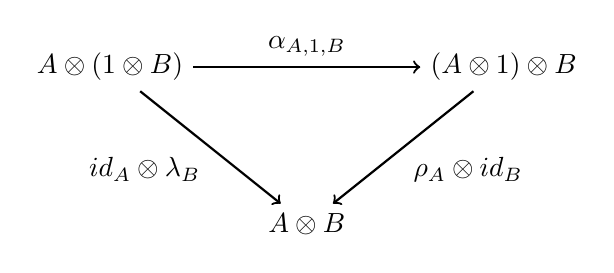
\begin{tikzpicture}
	\node (1) {$A\otimes (1\otimes B)$};
	\node (2) [right of=1] {};
	\node (3) [right of=2] {$(A\otimes 1)\otimes B$};
	\node (4) [node distance=2cm, below of=2] {$A\otimes B$};
	
	\draw [-to] (1) to node {$\alpha_{A, 1, B}$} (3);
	\draw [-to] (1) to node [swap]{$id_A\otimes \lambda_B$} (4);
	\draw [-to] (3) to node {$\rho_A\otimes id_B$} (4);
\end{tikzpicture}
\end{center}

\begin{center}
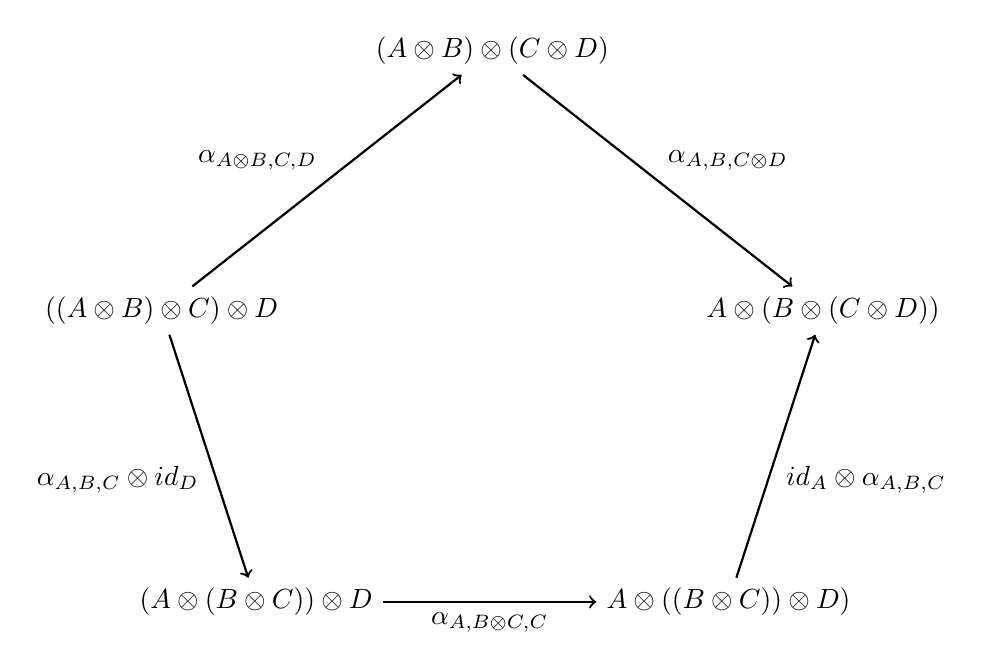
\begin{tikzpicture}
	\node (C) {};
	\node (1) [node distance=3.3cm, above of=C] {$(A\otimes B)\otimes (C\otimes D)$}; 
	\node (2) [node distance= 4.2cm, left of=C] {$((A\otimes B)\otimes C)\otimes D$};	
	\node (3) [node distance= 4.2cm, right of=C] {$A\otimes (B\otimes (C\otimes D))$};
	
	\node (D) [node distance=3.7cm, below of=C] {};
	\node (4) [node distance= 3cm, left of=D] {$(A\otimes (B\otimes C))\otimes D$};
	\node (5) [node distance= 3cm, right of=D] {$A\otimes ((B\otimes C))\otimes D)$};
	
	
	\draw [-to] (2) to node {$\alpha_{A\otimes B, C, D}$} (1);
	\draw [-to] (1) to node {$\alpha_{A, B, C\otimes D}$} (3);
	\draw [-to] (2) to node [swap]{$\alpha_{A, B, C}\otimes id_D$} (4);
	\draw [-to] (4) to node [swap]{$\alpha_{A, B\otimes C, C}$} (5);
	\draw [-to] (5) to node [swap]{$id_A\otimes \alpha_{A, B, C}$} (3);
\end{tikzpicture}
\end{center}

\begin{center}
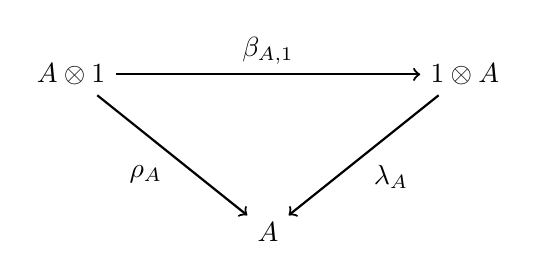
\begin{tikzpicture}
	\node (1) {$A\otimes 1$};
	\node (2) [right of=1] {};
	\node (3) [right of=2] {$1\otimes A$};
	\node (4) [node distance=2cm, below of=2] {$A$};
	
	\draw [-to] (1) to node {$\beta_{A, 1}$} (3);
	\draw [-to] (1) to node [swap]{$\rho_A$} (4);
	\draw [-to] (3) to node {$\lambda_A$} (4);
\end{tikzpicture}
\end{center}

\begin{center}
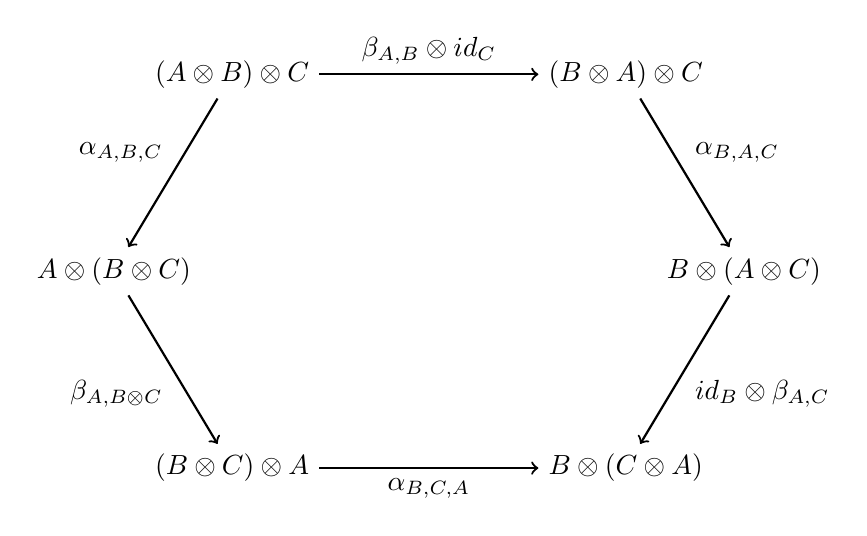
\begin{tikzpicture}
	\node (C) {};
	\node (1) [above of=C, left of=C] {$(A\otimes B)\otimes C$};
	\node (2) [above of=C, right of=C] {$(B\otimes A)\otimes C$};
	\node (3) [node distance=4cm, left of=C] {$A\otimes(B\otimes C)$};
	\node (4) [node distance=4cm, right of=C] {$B\otimes (A\otimes C)$};
	\node (5) [below of=C, left of=C] {$(B\otimes C)\otimes A$};
	\node (6) [below of=C, right of=C] {$B\otimes (C\otimes A)$};
	
	\draw [-to] (1) to node {$\beta_{A, B}\otimes id_C$} (2);
	\draw [-to] (1) to node [swap]{$\alpha_{A, B, C}$} (3);
	\draw [-to] (2) to node {$\alpha_{B, A, C}$} (4);
	\draw [-to] (3) to node [swap]{$\beta_{A, B\otimes C}$} (5);
	\draw [-to] (5) to node [swap]{$\alpha_{B, C, A}$} (6);
	\draw [-to] (4) to node {$id_B\otimes \beta_{A, C}$} (6);
\end{tikzpicture}
\end{center}

\begin{center}
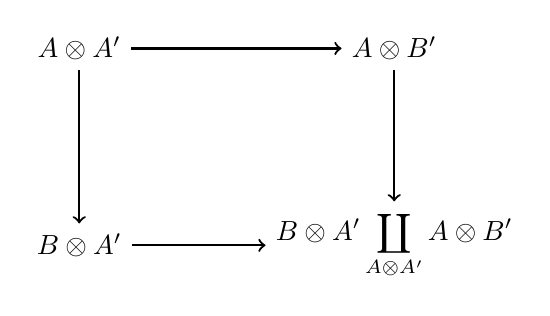
\begin{tikzpicture}
	\node (1) {$A\otimes A'$};
	\node (3) [below of=1] {$B\otimes A'$};
	\node (2) [node distance=4cm, right of=1] {$A\otimes B'$};
	\node (4) [below of=2] {${\displaystyle B\otimes A'\coprod_{A\otimes A'}A\otimes B'}$};

	\draw [-to] (1) to node {} (2);
	\draw [-to] (1) to node {} (3);
	\draw [-to] (2) to node {} (4);
	\draw [-to] (3) to node {} (4);	
\end{tikzpicture}
\end{center}

\begin{center}
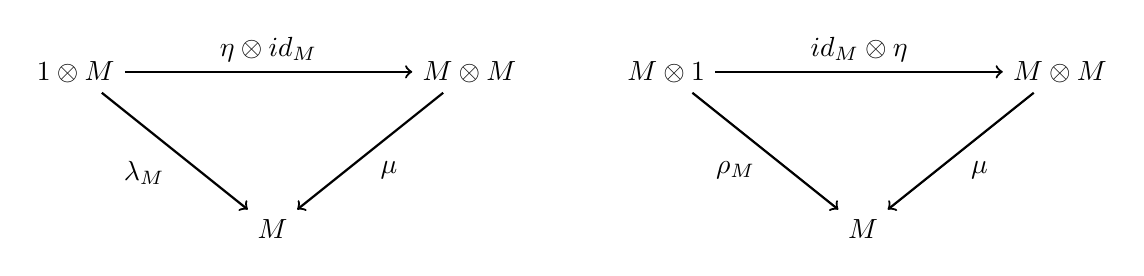
\begin{tikzpicture}
	\node (1) {$1\otimes M$};
	\node (2) [right of=1] {};
	\node (3) [right of=2] {$M\otimes M$};
	\node (4) [node distance=2cm, below of=2] {$M$};
	
	\node (5) [right of=3] {$M\otimes 1$};
	\node (6) [right of=5] {};
	\node (7) [right of=6] {$M\otimes M$};
	\node (8) [node distance=2cm, below of=6] {$M$};	
	
	\draw [-to] (1) to node {$\eta\otimes id_M$} (3);
	\draw [-to] (1) to node [swap]{$\lambda_M$} (4);
	\draw [-to] (3) to node {$\mu$} (4);
	
	\draw [-to] (5) to node {$id_M\otimes \eta$} (7);
	\draw [-to] (5) to node [swap]{$\rho_M$} (8);
	\draw [-to] (7) to node {$\mu$} (8);	
\end{tikzpicture}
\end{center}

\begin{center}
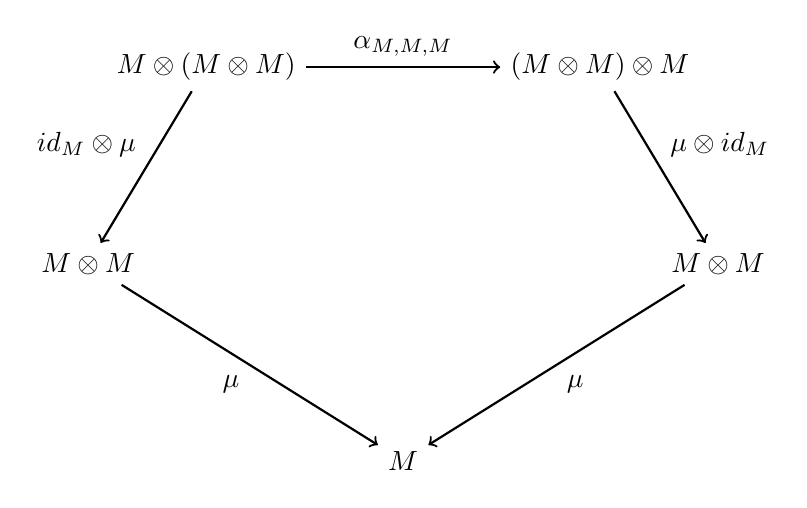
\begin{tikzpicture}
	\node (C) {};
	\node (1) [above of=C, left of=C] {$M\otimes (M\otimes M)$};
	\node (2) [above of=C, right of=C] {$(M\otimes M)\otimes M$};
	\node (3) [node distance=4cm, left of=C] {$M\otimes M$};
	\node (4) [node distance=4cm, right of=C] {$M\otimes M$};
	\node (5) [below of=C] {$M$};


	\draw [-to] (1) to node {$\alpha_{M, M, M}$} (2);
	\draw [-to] (1) to node [swap]{$id_M\otimes \mu$} (3);
	\draw [-to] (2) to node {$\mu\otimes id_M$} (4);
	\draw [-to] (3) to node [swap]{$\mu$} (5);
	\draw [-to] (4) to node {$\mu$} (5);	

\end{tikzpicture}
\end{center}

\begin{center}
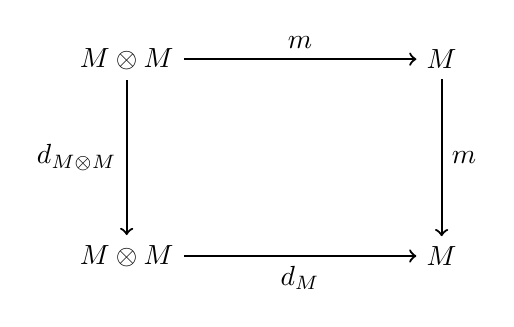
\begin{tikzpicture}
	\node (1) {$M\otimes M$};
	\node (3) [below of=1] {$M\otimes M$};
	\node (2) [node distance=4cm, right of=1] {$M$};
	\node (4) [below of=2] {$M$};

	\draw [-to] (1) to node {$m$} (2);
	\draw [-to] (1) to node [swap]{$d_{M\otimes M}$} (3);
	\draw [-to] (2) to node {$m$} (4);
	\draw [-to] (3) to node [swap]{$d_M$} (4);	
\end{tikzpicture}
\end{center}


\end{document}








